\section{Introduction}

% Reproducibility is more important than it is hard
The importance of reproducibility outweighs its difficulty. While wrestling with
large amounts of data, millions of lines of code, and diverse developer groups, it
is extremely  hard to remember to make workflows understandable, let alone
reproducible. But our research group has found  that the benefits of
reproducibility, from a research, educational, and productivity standpoint,
make the pain points worth it. After all, the scientific method requires such
practices to do science and other fields have been emphasizing the
reproducibility of experimental results for {\it centuries}; it is about time
that the field of computer systems change its {\it ad-hoc} workflows to be more
reproducible.

% Not incentivized
Once we adopted this philosophy, the road to reproducible research and paper
artifacts was not smooth.  We use the Popper
convention~\cite{jimenez:ipdpsw17-popper} because of its focus on open-source
cluster management toolkits. We have produced four Popper-compliant papers, as
shown in Table~\ref{table:papers}. We also note the status of the
Popper-compliance, where GOLD means that results are fully reproducible, PASS
means the experiments will run, and FAIL means that experiments are not
guaranteed to execute~\cite{jimenez:rr18-popper}. A FAIL status is still
Popper-compliant because experiment artifacts and results are available.

\begin{table}[t]
\centering
\normalsize
\begin{tabular}{ >{}m{2.8in} | c }
\multicolumn{1}{c|}{Paper [Reference]} & Status \\ \hline
&\\
Malacology: A Programmable Storage System~\cite{sevilla:eurosys17-malacology} & PASS\\ 
&\\\hdashline
&\\
Cudele: An API and Framework for Programmable Consistency and Durability in a Global Namespace~\cite{sevilla:ipdps18-cudele} & GOLD \\
&\\\hdashline
&\\
Programmable Caches with a Data Management Language \& Policy Engine~\cite{sevilla:ccgrid18-parsplice} & FAIL \\
&\\\hdashline
&\\
Tintenfisch: File System Namespace Schemas and Generators~\cite{sevilla:techreport18-tintenfisch} & GOLD \\
\end{tabular}

\caption{Papers following the Popper Convention. The statuses are
from~\cite{jimenez:rr18-popper}, where PASS means experiments run, GOLD means
results are reproducible, and FAIL means experiment artifacts are available
(but may not run). Over time, our Popper-compliance has improved, except for
the work we did in~\cite{sevilla:ccgrid18-parsplice}, which faced security
obstacles (see Section~\S\ref{sec:reqs}).}

\label{table:papers}
\end{table}

% Contributions
While our experience with these state-of-the-art
devops tools have been delightfully straightforward, which is no doubt a
testament to the importance of reproducibility in real, large-scale clusters,
our struggle composing these tools together in a coherent way has been the real
challenge.  From designing workflows with these tools, we have developed a list
of pitfalls that wasted time and effort. Our contributions are as follows:

\begin{itemize}

  \item the structure and workflow of some of our Popper-compliant papers,
using a baseline template designed for the Ceph~\cite{weil:osdi2006-ceph}
storage system (Section~\S\ref{sec:popper-compliant-papers}).

  \item three pitfalls for Popper-compliant papers that severely limited
productivity in early papers; designing best practices that address these
pitfalls before starting the project saved us time and effort in subsequent
Popper-compliant papers (Section~\S\ref{popper-best-practices}).

  \item a call to arms for the downfall of practices that fly in the face of
Popper-compliance. We highlight difficulties with academic conferences, work at
national laboratories, and work in industry because that is where we have the
most experience (Section~\S\ref{sec:community-cooperation}).

\end{itemize}

Over time, our Popper status has improved from PASS to GOLD. The FAIL status
can be attributed to security issues working at a national laboratory, as
described in more detail in Section~\S\ref{sec:reqs}. We also note that going
back and making published papers Popper-compliant is too difficult and is not
incentivized, as described in Section~\S\ref{sec:repro}. It is our hope that
the pitfalls stumbled over can be used as a best practices guide for future
articles.

\section{Popper-compliant Papers}
\label{sec:popper-compliant-papers}

We use the reader/reviewer sample workflow outlined
in~\cite{jimenez:ipdpsw17-popper} and shown in Figure~\ref{fig:workflow}. For
the visualization component (1), we use Jupyter notebooks. The notebooks
themselves are versioned with Git and users interact with local copies by
cloning the repository and launching a Jupyter Docker container. The paper is
written in \LaTeX and built with a Docker container.  For the code component
(2), both the source code for the system itself and the deploy/experiment code
is stored on GitHub. When running experiments, we use Docker containers to
isolate libraries and binaries. For the multi-node component (3), we use
CloudLab machines and Ansible to script deployment and experiment
orchestration. For the data set components (4), we use GitHub to store results
files; our inputs and results are small enough that we do no need a larger
capacity.  GitHub allows files up to 50MB and stores data on S3.

\begin{figure}[tb] 
  \centering
  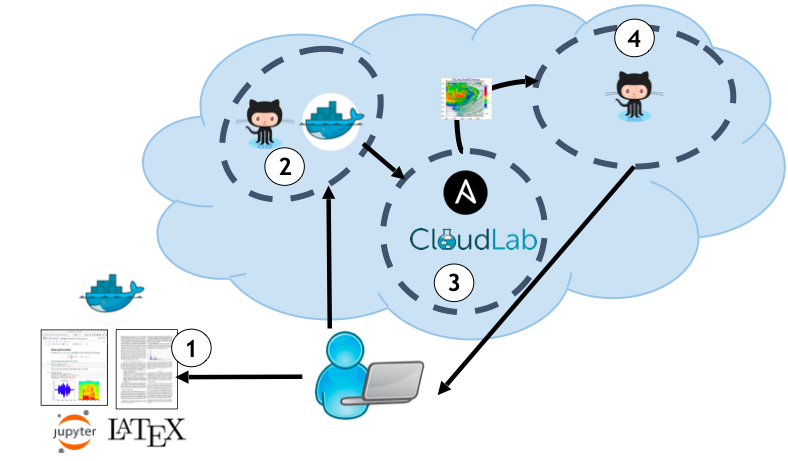
\includegraphics[width=1\linewidth]{./figures/workflow.png}
  \caption{Illustration of the Popper workflow used in our papers; Figure is
adapted from~\cite{jimenez:ipdpsw17-popper}. For (1) - the visualization
component - we use Jupyter, \LaTeX, and Docker; for (2) - the code component -
we use GitHub and Docker; for (3) - the multi-node component - we use Ansible
and CloudLab; and for (4) - the data set component - we use GitHub.}
  \label{fig:workflow}
\end{figure}

Our experiments start with a baseline; to describe the process, we reference
our
ceph-popper-template\footnote{https://github.com/michaelsevilla/ceph-popper-template}
set up on CloudLab. Users setup SSH keys and deploy CloudLab nodes using our
CephFS Profile \footnote{https://www.cloudlab.us/p/CephFS/CephFS-HEP}.  The
profile has the nodes automatically install Docker on bootup using our
install\footnote{https://github.com/michaelsevilla/ceph-popper-template/blob/master/hardware/cloudlab/install.sh}
script. After the nodes finish booting ({\it i.e.}  their status on the
CloudLab GUI read as READY), users push SSH keys using a convenience
script\footnote{https://raw.githubusercontent.com/michaelsevilla/ceph-popper-template/master/hardware/cloudlab/pushkeys.sh}.

The deploy code is based on
ceph-ansible\footnote{https://github.com/ceph/ceph-ansible/wiki}, a tool that
configures hardware and software for Ceph. We forked the project and made it
less dependent on Python. To run an experiment, users log in into the head node
and clone the ceph-popper-template. This repository has submodules that point
to ceph-ansible and our own custom roles; configuration files for our Ceph
setup; and helper scripts written in bash that deploy Ceph and run the
benchmarks. An outline of this organization is shown in
Figure~\ref{fig:expdir}.  For more information, see the
README\footnote{https://github.com/michaelsevilla/ceph-popper-template}. For
more information on the baseline and pipelines terminology, read more on the
Popper Convention \footnote{http://falsifiable.us/}. Then users configure their
cluster by specificing IPs and user names in the \texttt{hosts} file. 

\begin{figure}[tb] 
  \centering
  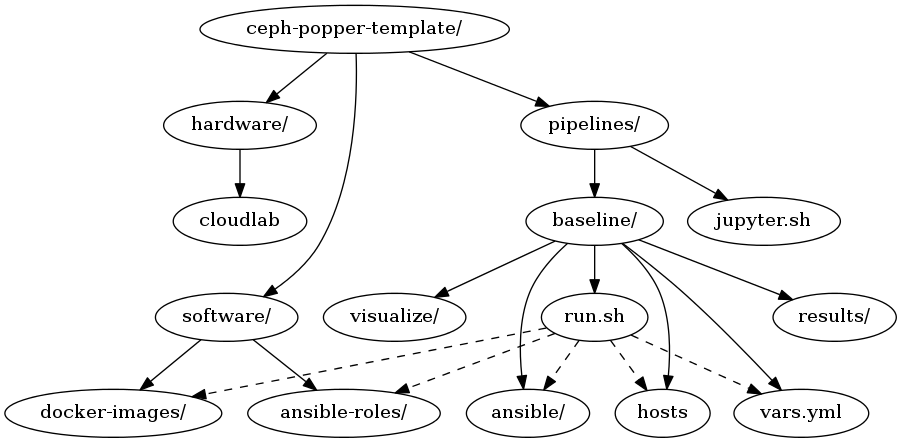
\includegraphics[width=1\linewidth]{./figures/expdir.png}
  \caption{Organization of our experiment directories. \texttt{baseline/} is an
example experiment and contains scripts populated with the Popper CLI. The
\texttt{run.sh} script uses many directories and files to setup and run
experiments, as indicated by the dashed lines.}
  \label{fig:expdir}
\end{figure}



Finally, users specify the Ceph services that should be deployed using the
\texttt{ansible/}\footnote{https://github.com/michaelsevilla/ceph-popper-template/tree/master/pipelines/baseline/ansible}
directory. This directory has code for deploying Ceph and its components:
\texttt{ansible.cfg}, \texttt{ceph.yml}, \texttt{cleanup.yml},
\texttt{group\_vars}, \texttt{monitor.yml}, and \texttt{workloads}. The *.yml
files are Ansible playbooks that start and configure components: ceph.yml
starts Ceph, cleanup.yml tears Ceph down, and monitor.yml starts daemons that
monitor performance. We separate these components into different playbooks so
users can mix and match Ceph services. The workloads directory has scrips for
running the baseline benchmarks. The other files and directories are Ansible
configuration files used by the playbooks.

Users can change the ansible/ceph.yml to specify which Ceph daemons to launch
in the cluster. It uses the hosts file we set up above and is based off the
ceph-ansible site file. High level configurations are in the vars.yml. This
file is heavily commented. For CloudLab, uncomment all blocks labeled
``Uncomment for CloudLab".

To configure the Ceph cluster with the variables in the Ceph configuration file
documentation
\footnote{http://docs.ceph.com/docs/jewel/rados/configuration/ceph-conf/},
change the Ansible \texttt{group\_vars/all} file. We also need to specify the
Docker image. These can be specified in each configuration file for the daemon
but for simplicity we put everything in the global variable file. Finally,
users run the \texttt{run.sh} script. 

\section{Popper Best Practices}
\label{popper-best-practices}

To produce Popper-compliant papers, we needed to change our workflows and
experimental procedures. We have learned the following lessons:

\subsection{Reproducibility Must Be a 1st Class Citizen}
\label{sec:repro}

% exploration vs. complete
Popper-compliance must be observed {\it throughout} the paper-writing process.
Attempts to make published papers Popper-compliant failed for three reasons:
(1) there is no incentive from the perspective of a graduate student, (2) it is
too hard to remember the experimental workflow, and (3) the artifacts cannot be
added to the camera-ready article. This introduces a careful design decision:
how does the user decide which results are exploratory and which are complete;
we do not want to waste space by saving results that do not contribute to the
paper but, at the same time, how do we know when an experiment is worthy of
being included in the paper? Discipline must be exercised throughout the paper-writing
process to make any experiment that we find useful must be immediately polished
to be Popper-compliant.

% cross-cluster compatibility 
Another pitfall we face is cross-cluster compatibility. After identifying
results as being useful, we usually find inventory files hard-coded throughout
the tree, configuration files randomly propagated to different directories,
visualization files reliant on data specified with hard-coded paths, and graphs
are not created automatically. To address this, we must exercise discipline to
separate cluster-specific files from cluster-agnostic files; we do this with
\texttt{configs\_*/} directories in our ceph-popper-template repository.

% organized repos/docs
Finally, organization and documentation must be required throughout the
paper-writing process. We fail to do this in early papers and this causes the
most work later on. System and experiment deploy code is rarely
self-explanatory. At a minimum, each experiment directory must contain a README
specifying how to run the jobs. To address this, we recommend relying heavily
on DockerHub, GitHub, and collaboration; making things public incentives
tidiness and organization. Using internal Docker or Git repositories hampers
Popper-compliance and discourages community involvement.

\subsection{Well-Defined Collaboration Roles}

% keeping organization workflows
Collaboration obviously speeds up code development and, As stated in the
previous section, collaboration can be used as motivation to keeping
Popper-compliant repositories; but collaboration can also hamper the process.
Researchers have different workflows and preferences. Committing system and
experimental deploy code with different toolkits, documentation, and styles to
the same repository results can result in a confusing organizational structure.
To address this, we recommend that the first author of the paper (1) produce a
style guide, either by committing a couple of experiments or adding detailed
READMEs and (2) act as the gatekeeper for all code. We recommend using GitHub
because it nicely formats READMEs and supports pull requests, issue trackers,
and project boards. Rather than having meetings to agree on experiment
organization, we recommend iteratively combining code from collaborators with
pull requests so the repository grows organically and quickly in the style
approved by the first author.

% merge conflicts
Another obstacle of collaboration is merge conflicts, especially when editing
the paper. We used to assign locks to people, in an {\it ad hoc} fashion over
email; this is not scalable. Instead, we now use Git to manage conflicts.
Before issuing a pull request, which notifies the first author, GitHub will
notify committers of changes they made in parallel with other changes. Our
policy is to force committers to resolve these merge conflicts before bothering
the first the author. While we still recommend issuing pull requests to make
sure the first author approves of the style, the merge conflicts workflow has
been an effective way to avoid annoying the first author with destructive
changes.

\subsection{Maintaining Pointers}

Popper-compliant papers provide pointers to graph artifacts, including results,
input files, and deploy code. But these links are problematic because they must
be maintained over time, even years after the paper is published. We have had
trouble maintaining these pointers because they (1) are ephemeral, (2) include
pointers to other repositories, and (3) include pointers to different
repository hosting sites.

%wary of ephemeral links
Ephemeral links and making sure that pointers are live is our biggest pain
point. Small, seemingly benign changes end up confusing users wanting to
reproduce our code. This is an artifact of how the internet was built, but
making sure that these links are live is one of the hardest challenges for
Popper-compliancy. To combat this, we suggest maintaining continuous
integration pipelines that read the paper source code and send REST requests to
websites to ensure that 404 codes are not returned.

%large code bases large code bases (src, deploy)
Pointers to other repositories can make the Popper-compliant repository
confusing and difficult to navigate. For example, our Cudele paper had Git
submodule pointers to 3 other GitHub repositories: one for Ansible deployment
code for Ceph, one for Ansible deployment code for monitoring code written by
our research lab, and one for our paper bibliography. Users unfamiliar with
Ansible or \LaTeX would have trouble understanding navigating large code bases;
but this practice is necessary to avoid duplicating functionality and ensuring
future-proof modules. Our recommendation for addressing this problem is
minimize the number of repository pointers and to document them thoroughly,
including the reasons that the pointer is necessary and what the other
repository does.

%different registry hubs (Docker, GitHub)
Finally, pointers to different repository sites can make Popper-compliant
papers difficult to understand. Again, this is a necessary evil because
research systems can be large and complicated with many moving parts. For
example, our Cudele paper uses a GitHub repository to maintain our source code
for our modified Ceph version, a GitHub repository to maintain our paper and
deploy code, a GitHub repository to maintain our common deploy code modules
(for monitoring), a DockerHub repository for housing software images with
compiled binaries for our source code of our modified Ceph version, and a
CloudLab repository to house our base images. Again, the recommended solution
for maintaining this complicated web of registry hubs is to thoroughly document
the process.

\subsection{Baselines}
% can't always have our own cluster
% continuous integration is hard
% baselines take time 

\section{Community Cooperation}
\label{sec:community-cooperation}

We have shown and described reproducibility pitfalls, but equally important is
community buy-in. Next, we outline practices that have been detrimental to our
Popper-compliance initiatives.

\subsection{Conference Requirements}

% double blinded; multiple revision rounds
The most common obstacle to our Popper-compliance efforts is double blinded
submissions. The process is a burden, as we must create anonymous repositories
and remove graph artifacts, but also blocks communication between researchers
and reviewers. Providing evidence that the experiments work confidently gives
credence to the experiment and allows reviewers the chance to examine
experiment parameters more closely. We go a step further and propose removing
all anonymity from the review process, facilitating a communication channel
between researchers and reviewers with the sole intent of improving the quality
of the paper. We applaud efforts of SC'18, IPDPS'18, and ASPLOS'18 as they move
towards this approach with multiple revision rounds, but argue for more
transparent review processes. We are encouraged that in the review of the
Cudele paper, one of the reviewers specifically asked for source code and
reproducibility artifacts; at that point, we gladly made Popper source links
available.

% clear definition of reproducibility, replicability, and open source
A second obstacle is that many conferences lack a clear definition of
reproducibility and replicability, which confuses submitters and reviewers
alike. One conference we were rejected from had reviewers that posited that our
paper reproducibility artifacts were out of scope while the submission website
clearly had our definition of reproducibility. This confusion is frustrating
and can lead to contentious reviews and rebuttals To remedy the situation, we
recommend emphasizing reproducibility initiatives to reviewers, even going as
far as to reward papers that have clearly thought about reproducibility.

\subsection{Industry/Laboratory Requirements}
\label{sec:reqs}

% private/propriety systems --> open architectures
We understand the monetary incentives to propriety systems but working with
code in these environments severely hampers our ability to make papers
Popper-compliant. Our experience in industry, which is by no means
representative of other companies, was to keep all code repositories private.
Furthermore, many companies have multiple repositories because development
teams like using version control systems ({\it e.g.}, git or svn) and hosting
services ({\it e.g.}, GitHub, GitLab, etc.) that they are familiar with. In
larger companies that acquire startups, this is a big problem as every group of
injected developers brings new ways of managing code.  Obviously, this makes
Popper-compliance impossible, except in a general sense.  We recommend that
companies adopt a unified version control system and make it public.

% support from upper level management for this process
Another obstacle to Popper-compliance is security. Many systems in national
laboratories require clearance and access is only granted to US citizens. In
fact, many systems are not even connected to the internet to discourage contact
with the outside world. While laboratories are expected to be research havens,
their priorities are obviously security over open research practices.

\section{Conclusion}

We have 
